\chapter{Introduction}
\label{chp:introduction}
Tribler is a peer-to-peer BitTorrent client that attempts to fully decentralize downloading, uploading and streaming of content.

Tribler focusses on the following goals:
\begin{itemize}
    \item Allow for secure and private communication and sharing of data.
    \item Enforce user contribution in the network
    \item Make it impossible to shut Tribler down, unless the Internet itself as a whole gets taken down.
\end{itemize}

A fully decentralized ecosystem i.e. no central components present, is Tribler's approach to achieve these goals.
Tribler has been designed and build with this focus~\cite{Pouwelse-tribler,Bakker-tribler}.
A distributed network requires both the presence and collaboration of participants, called peers, to be able to achieve this.

This thesis was conducted to improve the connectability and overall performance of Tribler, by identifying and removing bottlenecks present in the system.

% \begin{figure}
%	\centerline{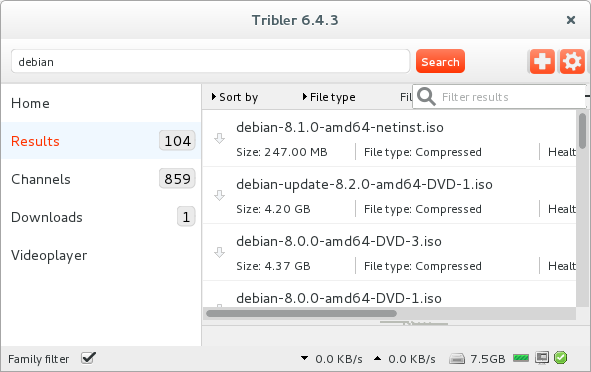
\includegraphics[scale=0.6]{introduction/figs/tribler-screenshot.png}}
%	\caption{Screenshot of Tribler v6.4.3.}
%	\label{fig:tribler-screenshot}
%\end{figure}

\section{BitTorrent protocol}
When sharing files by using the BitTorrent protocol, a peer that uploads parts of a file to another peer, is called a seeder.
A peer that is downloading a file of a seeder is called a leecher.
Any peer can be both a seeder and leecher at the same time, and join the network at any given time.

The ratio between the total data downloaded and uploaded is called the seeding ratio \cite{Cohen-bittorrent}.
The seeding ratio can be seen as an indication of the level of collaboration i.e. giving back resources to the network.

Seeding can be seen as an interaction between peers, where the seeder aids the leeching peer.
By utilizing the seeders upload bandwidth, the leeching peer can use his download bandwidth to download a file.
While there is a clear incentive for the leecher by downloading the desired file, there is none for the seeder.
Especially since the leecher has a little chance of becoming also be a seeder for the original seeder \cite{Lai-Incentives}.

Having peers actively and persistently contribute to the network will increase the network's health which in turn provides several benefits for all peers.
A more healthy network results in a higher availability of seeders and results in high download speeds.
It has been shown that private communities where the seeding ratio is high, provides better download conditions \cite{meulpolder-privatecommunities}.
In these private communities, trackers i.e. central components introduce peers to each other using the Tit-for-tat approach \cite{cohen-titfortat}.
The Tit-for-Tat approach is aiding peers who have aided you in the past,
The absence of trackers, which is often the case in public networks, results in free-riding \cite{Adar-Freeriding}.
A free-riding peer does not or gives little back to the network while receiving all benefits i.e. download without any restriction.
\todo{Explain the optimistic chocking approach.}BitTorrent applies a variation of the Tit-for-tat strategy, optimistic chocking, to combat this problem.
The Tit-for-Tat strategy is to only provide help to peers that return this help.
However, it has been shown that this approach is not effective in battling abuse \cite{Pouwelse-tribler}.

\section{Tribler}
Tribler wants to achieve a high global seeding ratio by making it beneficial to have such a ratio.
Nodes can award each other with higher cooperation if a node has a reputation of being cooperative,
while malicious nodes are prevented from tampering and freeriding.
Within Tribler anonymous connections have been implemented recently using onion routing~\cite{Plak-anonymous,ruigrok-anonymous,tanaskoski-anonymous}.
This feature allows downloaders to become indistinguishable from other users in the network save guarding their privacy.
Every data packet has to be forwarded
by a number of intermediate hops between the leecher and seeder~\cite{Plak-anonymous,tanaskoski-anonymous}.
The total cost of bandwidth per file is increased,
because it has to be forwarded by multiple nodes.
but also the number of nodes helping a single node downloading a file increases.
The increase in nodes working together increases the necessity of an incentive system to reward collaboration.

Dispersy is middleware for data dissemination in a network.
Dispersy is used heavily within Tribler and is maintained by the Tribler organisation.
Our work is build upon Dispersy.
Dispersy is used to exchange data between two specific nodes~\cite{zeilemaker-dispersy}.
Functionality was added to Dispersy during the thesis.
The additions are described in chapter \ref{chapt:design}.

\section{Objective and research questions}
\label{chp1:sct:objectives-research-questions}
The objective of this thesis is to improve the connectability, speed and responsiveness of Tribler. Furthermore, this thesis focusses on removing (CPU and IO) bottlenecks present.
Moreover, these improvements will be applied by means of refactoring current code, which is largely undocumented, unnecessary complex and has little structure.
In general, projects facing similar issues can learn from and integrate the decision and changes made to the Tribler code base.

The research presented in this thesis was carried out in cooperation with the Tribler team. 
The Tribler team consists of both staff of the Technical University of Delft and Bachelor and Master students.
Both staff and students have been working for years on Tribler and know parts of Tribler in detail.
Using this knowledge resulted in a shorter learning trajectory to understand Tribler's code base and identify problem areas related to the objective of this thesis.
Based on the objectives of Tribler, this thesis aims to answer the main research question formulated below.\\

\noindent
\textbf{Main Research Question:} How can we improve Tribler's performance and code base by means of asynchronous programming and refactoring?\\

To answer the main research question, we have defined three research questions below. Each of these research questions will be justified as why they contribute to the main research question.\\

\noindent
\textbf{Research Question 1:} How can we identify bottlenecks in a complex system such as Tribler?\\

Software projects such as Tribler have many lines of code (LOC). 
They are often dependant on libraries i.e. third party code and combine several components or modules to form a single entity i.e. a program.
To improve such an entity, one needs to be able to identify bottlenecks that are the root of limitations.
Such limitations may manifest themselves in the form of e.g. poor performance or bad responsiveness.
Identifying these bottlenecks is the first step to resolve them.\\

\noindent
\textbf{Research Question 2:} Can a system such as Tribler benefit from asynchronous programming?\\

Asynchronous programming can improve the performance and responsiveness of a system, but it has its drawbacks. Identifying these drawbacks and deciding if the benefits outweigh the costs is necessary to prevent the current state from worsening. \\

\noindent
\textbf{Research Question 3:} How can a complex code base such as Tribler's be effectively refactored to reduce complexity while improving performance?\\

As we strive to make Tribler's code base less complex and easier for new members to get familiar with, identifying complex structures and means to refactor them in such a way that it reduces the complexity is needed.
This aids in new members being able to actively contribute to Tribler faster and easier.\

\section{Main contributions}
The main contribution this thesis offers are as follows. We present a method to identify bottlenecks in a complex system such as Tribler. Identifying bottlenecks is the first step of improving a system. While this thesis focusses on Tribler, similar approaches for different projects are possible.
Next, we provide arguments where asynchronous programming is preferred over synchronous programming and when it is not.
Finally, we present methods to reduce the complexity of a code base while improving performance and readability by using Tribler as a case study.


\section{Outline}
In this chapter we provided an introduction of the BitTorrent protocol and Tribler, presented the research questions this thesis aims to answer. This section describes the other chapters in this thesis and their relevance to the research questions provided in section \ref{chp1:sct:objectives-research-questions}.
Chapter \ref{chp:introduction} provides information on Tribler.
Chapter \ref{chp:problem-description} presents an overview of some of the problems Tribler is currently facing which this thesis addresses.
\todo{Add more here.}
